\documentclass[twoside]{book}

% Packages required by doxygen
\usepackage{fixltx2e}
\usepackage{calc}
\usepackage{doxygen}
\usepackage[export]{adjustbox} % also loads graphicx
\usepackage{graphicx}
\usepackage[utf8]{inputenc}
\usepackage{makeidx}
\usepackage{multicol}
\usepackage{multirow}
\PassOptionsToPackage{warn}{textcomp}
\usepackage{textcomp}
\usepackage[nointegrals]{wasysym}
\usepackage[table]{xcolor}

% Font selection
\usepackage[T1]{fontenc}
\usepackage[scaled=.90]{helvet}
\usepackage{courier}
\usepackage{amssymb}
\usepackage{sectsty}
\renewcommand{\familydefault}{\sfdefault}
\allsectionsfont{%
  \fontseries{bc}\selectfont%
  \color{darkgray}%
}
\renewcommand{\DoxyLabelFont}{%
  \fontseries{bc}\selectfont%
  \color{darkgray}%
}
\newcommand{\+}{\discretionary{\mbox{\scriptsize$\hookleftarrow$}}{}{}}

% Page & text layout
\usepackage{geometry}
\geometry{%
  a4paper,%
  top=2.5cm,%
  bottom=2.5cm,%
  left=2.5cm,%
  right=2.5cm%
}
\tolerance=750
\hfuzz=15pt
\hbadness=750
\setlength{\emergencystretch}{15pt}
\setlength{\parindent}{0cm}
\setlength{\parskip}{3ex plus 2ex minus 2ex}
\makeatletter
\renewcommand{\paragraph}{%
  \@startsection{paragraph}{4}{0ex}{-1.0ex}{1.0ex}{%
    \normalfont\normalsize\bfseries\SS@parafont%
  }%
}
\renewcommand{\subparagraph}{%
  \@startsection{subparagraph}{5}{0ex}{-1.0ex}{1.0ex}{%
    \normalfont\normalsize\bfseries\SS@subparafont%
  }%
}
\makeatother

% Headers & footers
\usepackage{fancyhdr}
\pagestyle{fancyplain}
\fancyhead[LE]{\fancyplain{}{\bfseries\thepage}}
\fancyhead[CE]{\fancyplain{}{}}
\fancyhead[RE]{\fancyplain{}{\bfseries\leftmark}}
\fancyhead[LO]{\fancyplain{}{\bfseries\rightmark}}
\fancyhead[CO]{\fancyplain{}{}}
\fancyhead[RO]{\fancyplain{}{\bfseries\thepage}}
\fancyfoot[LE]{\fancyplain{}{}}
\fancyfoot[CE]{\fancyplain{}{}}
\fancyfoot[RE]{\fancyplain{}{\bfseries\scriptsize Generated by Doxygen }}
\fancyfoot[LO]{\fancyplain{}{\bfseries\scriptsize Generated by Doxygen }}
\fancyfoot[CO]{\fancyplain{}{}}
\fancyfoot[RO]{\fancyplain{}{}}
\renewcommand{\footrulewidth}{0.4pt}
\renewcommand{\chaptermark}[1]{%
  \markboth{#1}{}%
}
\renewcommand{\sectionmark}[1]{%
  \markright{\thesection\ #1}%
}

% Indices & bibliography
\usepackage{natbib}
\usepackage[titles]{tocloft}
\setcounter{tocdepth}{3}
\setcounter{secnumdepth}{5}
\makeindex

% Hyperlinks (required, but should be loaded last)
\usepackage{ifpdf}
\ifpdf
  \usepackage[pdftex,pagebackref=true]{hyperref}
\else
  \usepackage[ps2pdf,pagebackref=true]{hyperref}
\fi
\hypersetup{%
  colorlinks=true,%
  linkcolor=blue,%
  citecolor=blue,%
  unicode%
}

% Custom commands
\newcommand{\clearemptydoublepage}{%
  \newpage{\pagestyle{empty}\cleardoublepage}%
}

\usepackage{caption}
\captionsetup{labelsep=space,justification=centering,font={bf},singlelinecheck=off,skip=4pt,position=top}

%===== C O N T E N T S =====

\begin{document}

% Titlepage & ToC
\hypersetup{pageanchor=false,
             bookmarksnumbered=true,
             pdfencoding=unicode
            }
\pagenumbering{roman}
\begin{titlepage}
\vspace*{7cm}
\begin{center}%
{\Large H\+C\+S\+R04 }\\
\vspace*{1cm}
{\large Generated by Doxygen 1.8.11}\\
\end{center}
\end{titlepage}
\clearemptydoublepage
\tableofcontents
\clearemptydoublepage
\pagenumbering{arabic}
\hypersetup{pageanchor=true}

%--- Begin generated contents ---
\chapter{Hierarchical Index}
\section{Class Hierarchy}
This inheritance list is sorted roughly, but not completely, alphabetically\+:\begin{DoxyCompactList}
\item \contentsline{section}{distance\+Sensors}{\pageref{classdistance_sensors}}{}
\begin{DoxyCompactList}
\item \contentsline{section}{sonar\+Sensor}{\pageref{classsonar_sensor}}{}
\end{DoxyCompactList}
\end{DoxyCompactList}

\chapter{Class Index}
\section{Class List}
Here are the classes, structs, unions and interfaces with brief descriptions\+:\begin{DoxyCompactList}
\item\contentsline{section}{\hyperlink{classdistance_meter}{distance\+Meter} }{\pageref{classdistance_meter}}{}
\item\contentsline{section}{\hyperlink{class_guard_object}{Guard\+Object} }{\pageref{class_guard_object}}{}
\item\contentsline{section}{\hyperlink{classparking_sensor}{parking\+Sensor} }{\pageref{classparking_sensor}}{}
\item\contentsline{section}{\hyperlink{classradar}{radar} }{\pageref{classradar}}{}
\end{DoxyCompactList}

\chapter{Class Documentation}
\hypertarget{classdistance_sensors}{}\section{distance\+Sensors Class Reference}
\label{classdistance_sensors}\index{distance\+Sensors@{distance\+Sensors}}


\hyperlink{classdistance_sensors}{distance\+Sensors} Class  




{\ttfamily \#include $<$distance\+Sensors.\+hpp$>$}

Inheritance diagram for distance\+Sensors\+:\begin{figure}[H]
\begin{center}
\leavevmode
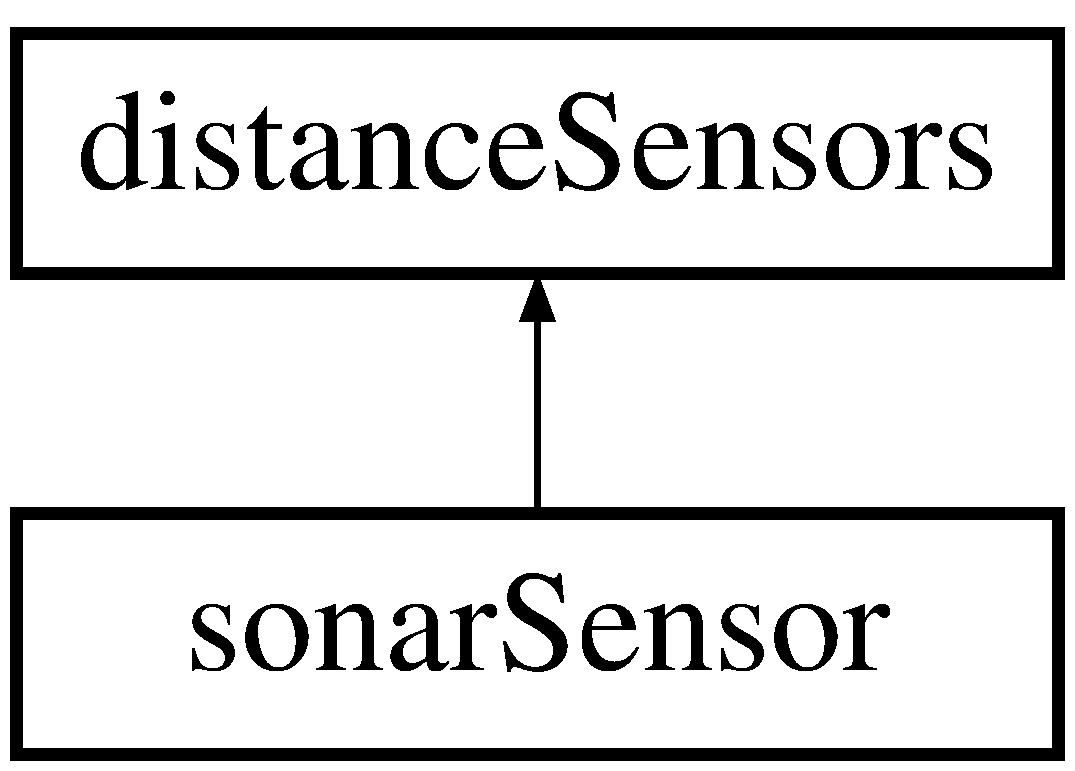
\includegraphics[height=2.000000cm]{classdistance_sensors}
\end{center}
\end{figure}
\subsection*{Protected Member Functions}
\begin{DoxyCompactItemize}
\item 
virtual int {\bfseries Ms\+Distance} ()\hypertarget{classdistance_sensors_a671c14e0869febbbcc4f428ee7bf0790}{}\label{classdistance_sensors_a671c14e0869febbbcc4f428ee7bf0790}

\end{DoxyCompactItemize}


\subsection{Detailed Description}
\hyperlink{classdistance_sensors}{distance\+Sensors} Class 

The super class for sensors, handy if there are more sensors added in the future. 

The documentation for this class was generated from the following file\+:\begin{DoxyCompactItemize}
\item 
distance\+Sensors.\+hpp\end{DoxyCompactItemize}

\hypertarget{classsonar_sensor}{}\section{sonar\+Sensor Class Reference}
\label{classsonar_sensor}\index{sonar\+Sensor@{sonar\+Sensor}}


\hyperlink{classsonar_sensor}{sonar\+Sensor} class  




{\ttfamily \#include $<$sonar\+Sensor.\+hpp$>$}

Inheritance diagram for sonar\+Sensor\+:\begin{figure}[H]
\begin{center}
\leavevmode
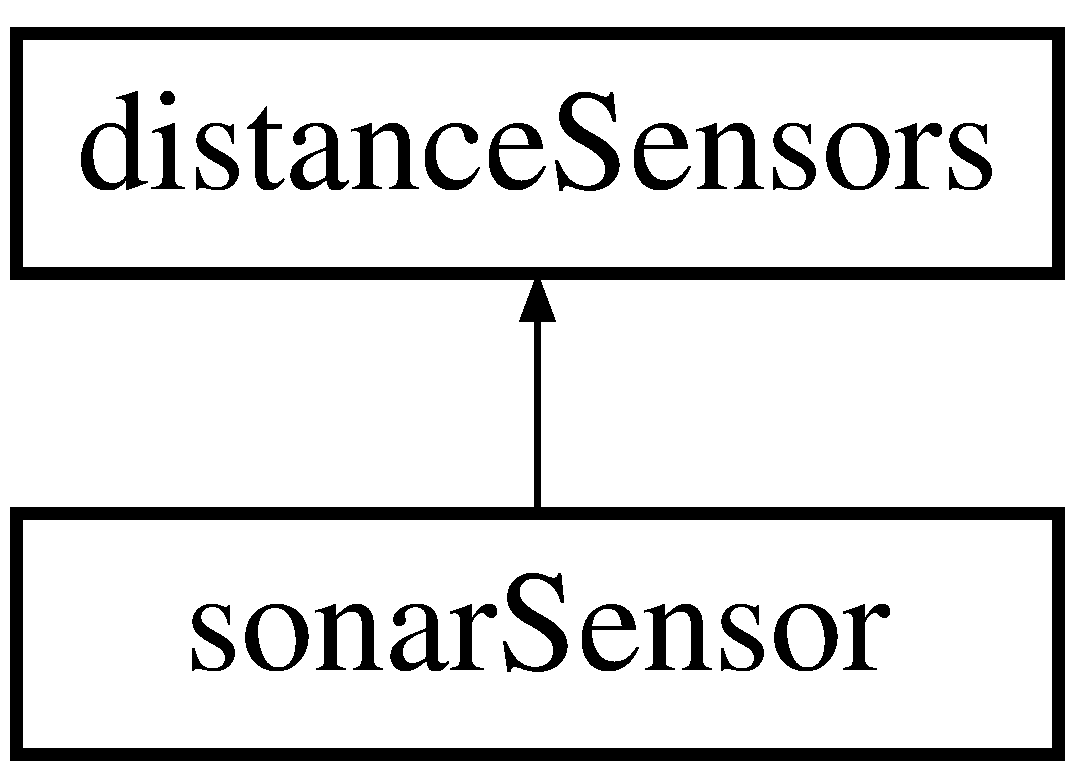
\includegraphics[height=2.000000cm]{classsonar_sensor}
\end{center}
\end{figure}
\subsection*{Public Member Functions}
\begin{DoxyCompactItemize}
\item 
\hyperlink{classsonar_sensor_a66bd7c088348ffe7b0e27186f5a6cc4e}{sonar\+Sensor} (hwlib\+::target\+::pin\+\_\+out \&p\+\_\+trigger, hwlib\+::target\+::pin\+\_\+in \&p\+\_\+echo)
\begin{DoxyCompactList}\small\item\em \hyperlink{classsonar_sensor}{sonar\+Sensor} Constructor \end{DoxyCompactList}\item 
int \hyperlink{classsonar_sensor_a2f58277f0b54053e8a3da2e43ee29560}{Ms\+Distance} ()
\begin{DoxyCompactList}\small\item\em Ms\+Distacne; int. \end{DoxyCompactList}\item 
bool \hyperlink{classsonar_sensor_a98b71611568b818f62a570c40daf56a5}{Trigger} (int Minimal\+Distance, int Maximum\+Distance, bool Set\+Constant\+Trigger=0)
\begin{DoxyCompactList}\small\item\em Trigger; boolean. \end{DoxyCompactList}\item 
int \hyperlink{classsonar_sensor_ae6bdf6cf320d32c07536ba86f8434d8e}{Trigger\+In\+Range} (int Minimal\+Distance, int Maximum\+Distance, bool Percentage\+Enable=0)
\begin{DoxyCompactList}\small\item\em Trigger\+In\+Range; int. \end{DoxyCompactList}\end{DoxyCompactItemize}
\subsection*{Additional Inherited Members}


\subsection{Detailed Description}
\hyperlink{classsonar_sensor}{sonar\+Sensor} class 

This class is used to initialize H\+C-\/\+S\+R04 sonar sensors. It may also be used by any similair sensor with the same pins and workings as the H\+C-\/\+S\+R04. The following is a short summary of the 3 functions this class provides\+: \hyperlink{classsonar_sensor_a2f58277f0b54053e8a3da2e43ee29560}{Ms\+Distance()}; \+: A function that measures the distance in Cm and returns an integer that is a 100 times larger for a more accurate number. \hyperlink{classsonar_sensor_a98b71611568b818f62a570c40daf56a5}{Trigger()}; \+: A function that returns a boolean value if it measures an object or being between two given values, it can be set to repeat. \hyperlink{classsonar_sensor_ae6bdf6cf320d32c07536ba86f8434d8e}{Trigger\+In\+Range()}; \+: A function that returns the value of a measurement inbetween two given values. It can also return a percentage int. 

\subsection{Constructor \& Destructor Documentation}
\index{sonar\+Sensor@{sonar\+Sensor}!sonar\+Sensor@{sonar\+Sensor}}
\index{sonar\+Sensor@{sonar\+Sensor}!sonar\+Sensor@{sonar\+Sensor}}
\subsubsection[{\texorpdfstring{sonar\+Sensor(hwlib\+::target\+::pin\+\_\+out \&p\+\_\+trigger, hwlib\+::target\+::pin\+\_\+in \&p\+\_\+echo)}{sonarSensor(hwlib::target::pin_out &p_trigger, hwlib::target::pin_in &p_echo)}}]{\setlength{\rightskip}{0pt plus 5cm}sonar\+Sensor\+::sonar\+Sensor (
\begin{DoxyParamCaption}
\item[{hwlib\+::target\+::pin\+\_\+out \&}]{p\+\_\+trigger, }
\item[{hwlib\+::target\+::pin\+\_\+in \&}]{p\+\_\+echo}
\end{DoxyParamCaption}
)}\hypertarget{classsonar_sensor_a66bd7c088348ffe7b0e27186f5a6cc4e}{}\label{classsonar_sensor_a66bd7c088348ffe7b0e27186f5a6cc4e}


\hyperlink{classsonar_sensor}{sonar\+Sensor} Constructor 

This constructor consists of 2 pins. Trigger\+: This pin is the signal that goes from the Arduino to the H\+C-\/\+S\+R04. It triggers the sensor to start a measurment cycle. Echo\+: This pin is the signal that goes from the H\+C-\/\+S\+R04 to the Arduino, the time it returns a high voltage can be translated into distance. It also includes the constructor from its super class. 

\subsection{Member Function Documentation}
\index{sonar\+Sensor@{sonar\+Sensor}!Ms\+Distance@{Ms\+Distance}}
\index{Ms\+Distance@{Ms\+Distance}!sonar\+Sensor@{sonar\+Sensor}}
\subsubsection[{\texorpdfstring{Ms\+Distance()}{MsDistance()}}]{\setlength{\rightskip}{0pt plus 5cm}int sonar\+Sensor\+::\+Ms\+Distance (
\begin{DoxyParamCaption}
{}
\end{DoxyParamCaption}
)\hspace{0.3cm}{\ttfamily [virtual]}}\hypertarget{classsonar_sensor_a2f58277f0b54053e8a3da2e43ee29560}{}\label{classsonar_sensor_a2f58277f0b54053e8a3da2e43ee29560}


Ms\+Distacne; int. 

Parameters\+: None. Variables\+: Counter = Starts at 0, is used to measure the time that has passed. Raw\+Distance = The return variabel. Is the distance in Cm$\ast$100. This function makes the H\+C-\/\+S\+R04 start a measurement cycle. It starts the cycle and adds 1 to the counter for every microsecond echo is high. It returns an int, which consist of the measured time echo was high divided by an amount that was based on real life testing. It is multiplied times 100 to make sure there is more accuracy in the measurement. 

Reimplemented from \hyperlink{classdistance_sensors}{distance\+Sensors}.

\index{sonar\+Sensor@{sonar\+Sensor}!Trigger@{Trigger}}
\index{Trigger@{Trigger}!sonar\+Sensor@{sonar\+Sensor}}
\subsubsection[{\texorpdfstring{Trigger(int Minimal\+Distance, int Maximum\+Distance, bool Set\+Constant\+Trigger=0)}{Trigger(int MinimalDistance, int MaximumDistance, bool SetConstantTrigger=0)}}]{\setlength{\rightskip}{0pt plus 5cm}bool sonar\+Sensor\+::\+Trigger (
\begin{DoxyParamCaption}
\item[{int}]{Minimal\+Distance, }
\item[{int}]{Maximum\+Distance, }
\item[{bool}]{Set\+Constant\+Trigger = {\ttfamily 0}}
\end{DoxyParamCaption}
)}\hypertarget{classsonar_sensor_a98b71611568b818f62a570c40daf56a5}{}\label{classsonar_sensor_a98b71611568b818f62a570c40daf56a5}


Trigger; boolean. 

Parameters\+: Minimal\+Distance, Maximum\+Distance, Set\+Constant\+Trigger Minimal\+Distance,Maximum\+Distance\+: Both in Cm. Gives us the range which to work with. Set\+Constant\+Trigger\+: Enables the while loop for constant measuring. Variables\+: max,min = Both are simply the parameters $\ast$100, because Ms\+Distance returns Cm $\ast$ 100. Keeping one standard helps with the math. Raw\+Distance = The return variabel from \hyperlink{classsonar_sensor_a2f58277f0b54053e8a3da2e43ee29560}{Ms\+Distance()}. Is the distance in Cm$\ast$100. Simple trigger returning 1 when triggered. Build-\/in while loop if needed. \index{sonar\+Sensor@{sonar\+Sensor}!Trigger\+In\+Range@{Trigger\+In\+Range}}
\index{Trigger\+In\+Range@{Trigger\+In\+Range}!sonar\+Sensor@{sonar\+Sensor}}
\subsubsection[{\texorpdfstring{Trigger\+In\+Range(int Minimal\+Distance, int Maximum\+Distance, bool Percentage\+Enable=0)}{TriggerInRange(int MinimalDistance, int MaximumDistance, bool PercentageEnable=0)}}]{\setlength{\rightskip}{0pt plus 5cm}int sonar\+Sensor\+::\+Trigger\+In\+Range (
\begin{DoxyParamCaption}
\item[{int}]{Minimal\+Distance, }
\item[{int}]{Maximum\+Distance, }
\item[{bool}]{Percentage\+Enable = {\ttfamily 0}}
\end{DoxyParamCaption}
)}\hypertarget{classsonar_sensor_ae6bdf6cf320d32c07536ba86f8434d8e}{}\label{classsonar_sensor_ae6bdf6cf320d32c07536ba86f8434d8e}


Trigger\+In\+Range; int. 

Parameters\+: Minimal\+Distance; int. Maximum\+Distance; int. Percentage\+Enable; int. Minimal\+Distance,Maximum\+Distance\+: Both in Cm. Gives us the range which to work with. Percentage\+Enable\+: Enables the return in percentages. Variables\+: max,min = Both are simply the parameters $\ast$100, because Ms\+Distance returns Cm $\ast$ 100. Keeping one standard helps with the math. Raw\+Distance = The return of Ms\+Distance. Is the distance in Cm$\ast$100. This function was mostly made for its percentage return making it very usefull for controls in games and other applications. The function returns a percentage within the trigger range with minimaldistance as baseline. 

The documentation for this class was generated from the following files\+:\begin{DoxyCompactItemize}
\item 
sonar\+Sensor.\+hpp\item 
sonar\+Sensor.\+cpp\end{DoxyCompactItemize}

%--- End generated contents ---

% Index
\backmatter
\newpage
\phantomsection
\clearemptydoublepage
\addcontentsline{toc}{chapter}{Index}
\printindex

\end{document}
